\chapter{Related Work}
\label{chapter:rw}

In this chapter it will be overviewed the work that has been done in the area of automatic prognostic and diagnostic. Diagnostic because,
 even though this thesis will be about prognosis, \cite{Hendriksen2013} states that the development, 
 validation and impact assessment of both cases can be mutatis mutandis applied. 

The prediction classification can be a diagnostic or a prognostic depending only on the amount of time until the outcome assessment. 
Being the options between the outcome assessment the present or the future, the former is a diagnostic and the latter a prognosis.

In the field of diagnosis the techniques used revolve around the same as in prognosis. Mainly it uses decision trees, artificial 
neural networks, association rules and Bayes classifiers as well as Support Vector Machines \cite{Kharya2012}.

There are three types of prediction that can be done when talking about prognosis:
\begin{itemize}
\item We can try to predict the probability of developing a disease or a state of that disease, in other words we can perform
 a risk assessment or predict the disease susceptibility;
\item We can predict if there will be recurrence of an event, for example if a cancer will recur after it was excised;
\item We can predict if the patient will be alive at a certain time point, known as \emph{survivability}. 

\end{itemize}

We will separate the review on prognostic prediction by disease in order to allow the comparison between the work being done in the various 
diseases. Showing that even though the same techniques are used they require different preprocessing and the end results are very data dependent.

We can find work on prognostic prediction as far back as 1980 \cite{Nash1980} where a regression analysis is used 
to find the predictive power of 17 features when predicting the survival of breast cancer patients. Also in the early
 90s \cite{Hanson1993} where logistic regression is used to predict Survival of HIV infected patients and
 \cite{Mangasarian1995} where dynamic programming is used to predict the time to recurrence of an excised cancer.
 
 \section{Alzheimer}
 \label{section:alz}
 
 % CHECK !!!! \hl[red]{Explicar que esta lista nao é extensiva... procurar mais alguns casos em papers da sara}
 
The Alzheimer’s disease (AD) is the most common form of dementia. It causes problems with memory, thinking and behavior. 
Symptoms usually develop slowly and get worse over time, becoming severe enough to interfere with daily tasks and eventually 
leading to death. In order to predict the progress of the disease several techniques have been applied.

Alzheimer’s disease is associated with variable but shortened life expectancy, even at relatively early stages. For that
 reason having a survivability expectancy might be important for the patients and their carers to understand and plan ahead. 

In \cite{Paradise2009} they used Cox proportional hazards regression modeling for univariate and multivariate statistics. 

On the multivariate analysis in order to find the most predictive features a forward stepwise approach was used followed
 by a backward stepwise linear regression in order to confirm if the results were robust. 

The final model, SAM (Survival in Alzheimer’s Model) is a 4 point risk scale according to whether a patient has or not the
 identified risk factors (increasing age, Constructional praxis, Gait apraxia). A patient with two risk factors will have 
 an 80\% chance of surviving 12 months, but less than 50\% chance of surviving 3.5 years.

This study has some limitations like the fact that one of the features where it was built upon, was clinically obtained, by a
 standardized assessment by the same doctor. Also this model’s generalizability may be limited because the cohort was a convenience
 sample and was not recruited to be representative of the larger population of people with AD.

In \cite{Zhou2011}, Zhou \emph{et al.} develop a new multi-task learning formulation based on the temporal group Lasso regularizer,
 in order to predict the Alzheimer’s disease progression, based on the Mini Mental State Examination (MMSE) and Alzheimer’s disease 
 Assessment Scale cognitive subscale (ADAS-Cog) scores, that give the cognitive status of a patient. The multi-task regression
 approach captures the relation of the task, and the regularizer ensures that a small set of features is used for the regression
 and that a large deviation between successive time points is penalized.

  \section{Cancer}
 \label{section:cancer}
 
Cancer, known medically as a malignant neoplasm, is a class of diseases characterized by out-of-control 
cell growth. It becomes harmful when faulted cells grow into lumps of tissue that are called tumors. The
 cancer may also end up by spreading when cancerous cells move through the lymphatic system or bloodstream.

Cancer is seen as a deadly disease, as most people end up dying from the cancer or its treatment. The ones 
that actually survive have twice the probability of developing a second cancer than the people that were never
 diagnosed with cancer. \cite{Rheingold2000}

Because of this the three types of prognosis are found in cancer research: there is the prediction of the
 probability of developing cancer, in other words we can perform a risk assessment or predict the cancer susceptibility,
 the prediction if there will be recurrence in the cancer after if it excised or the prediction if the patient will 
 be alive at a certain time point. 

In these three areas of prognosis we have the following work.

To perform the prediction of survival at 5, 10 and 15 years after the diagnostic, \cite{Lundin1999} uses artificial
 neural networks and logistic regression, showing that neural networks are consistent with logistic regression as is  represented in \ref{fig:LRvsNN}. 

\begin{figure}[!htb]
  \centering
  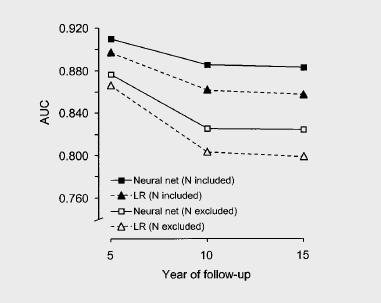
\includegraphics[width=0.75\textwidth]{Figures/LRvsNN.png}
  \caption{AUCs for the neural network and logistic regression (LR).}
  \label{fig:LRvsNN}
\end{figure}

In \cite{Steyerberg2005}, in order to decide which treatment is better for the patients’ well-being, a Cox regression analysis
 is used to predict a score based on the regression coefficients, which classifies the patients in 3 different groups: the ones
 with good, intermediate or bad prognosis in terms of survivability. Using this knowledge of the degree of prognosis in addition
 with the short-term versus long-term benefits of each treatment, a better choice can be performed helping to improve the patient’s quality of life. 

To predict the overall survivability, at 1 year and 5 years mark, of patients with Acute Myeloid Leukemia, Breems \emph{et al.} applied 
multivariate Cox regression analysis with stepwise backward selection on the patient’s age at the time of the relapse, length of relapse 
free interval, previous stem cell transplant and cytogenetics. 

Like in \cite{Steyerberg2005}, they used the regression coefficients has a score function that is used to classify the patients \cite{Breems2005}

The purpose of \cite{Delen2005} is to develop predictive models and discover/explain relationships between certain independent variables and the
 survivability, 5 years after the diagnosis, in the context of breast cancer. Delen \emph{et al.} per-form a comparative study with decision trees (C5.0),
 MLP neural network and logistic regression. Showing that with the SEER dataset and using a tenfold cross validation, the decision tree performed 
 the best out of the three with accuracy of 0.9362, closely followed by the neural network that achieved 0.9121 and the logistic regression that
 got 0.8920.

In the presence of microarray data, the clinical data is usually underused say Gevaert \emph{et al.} that in \cite{Gevaert2006} propose the usage of Bayesian 
networks to equally use both sources of data and that way get better results when performing the prognosis. 

They evaluated three methods for integrating clinical and microarray data: decision integration, partial integration and full integration 
and used them to classify publicly available data on breast cancer patients into a poor and a good prognosis group. The partial integration
 method is most promising and has an independent test set area under the ROC curve of 0.845.

In the problem addressed in \cite{Anagnostopoulos2006}, a neural network calculates a time interval that corresponds to a possible right
 end-point of the patient’s disease-free survival time, in other words it predicts the time to recur (TTR) by classifying the patient into 
 4 classes, TTR $\leq$ 1 year, TTR $\leq$ 3 years, TTR $\leq$ 6 years and TTR $>$ 6 years. The accuracy of the neural network was measured through a
 stratified tenfold cross validation approach. Sensitivity ranged between 80.5 and 91.8\%, while specificity ranged between 91.9 and 97.9\%,
 depending on the tested fold and the partition of the predicted period. 

In \cite{Bellaachia2006} a comparison is made between different data mining techniques, Naïve Bayes, Neural Networks and Decision Trees 
when predicting survivability of breast cancer patients 5 years after the diagnose. For that comparison the Weka toolkit\footnote{http://www.cs.waikato.ac.nz/ml/weka/} and the SEER 
Dataset is used, which is composed by demographic data (age, race, etc.) and clinical data (Extension of tumor, stage of cancer, etc.). 
After the tests the conclusion was that both, decision trees and neural networks, had better and similar performance with accuracy around 86\%, 
though in the computational time the approaches did differ where the neural networks model took 12 times more to be built.

Because of the neural networks’ ability to consider variable relations and create non-linear predictions models they are a very used 
method for cancer survivability prediction, how long after surgery it is expected that the cancer will recur. Here in \cite{Chi2007} it 
is shown that they can be used to predict the probability of survivability, and based on a threshold classify them as good or bad prognosis,
 with 2 different datasets. 

 In \cite{Endo2008}, Endo \emph{et al.} use Logistic Regression model, Artificial Neural Network (ANN), Naive Bayes, Bayes Net, and a collection of Decision Trees (Decision trees with naïve Bayes, ID3 and J48 algorithms) to predict breast cancer survival at 5 years learning that Logistic regression has the 
 highest accuracy along with J48. Decision trees tend to have high sensitivity. But is also shown that the best algorithm depends on the object
 and the dataset.

Because there is no use of fuzzy logic when performing cancer prognosis, most of the current work uses neural networks that yield difficult
 to understand models and that there is no use of hybridization of machine learning techniques, Muhammad Umer Khan \emph{et al.} investigated a hybrid
 scheme based on fuzzy logic and decision trees on the SEER dataset. They performed experiments using different combinations of number of 
 decision tree rules, types of fuzzy membership functions and inference techniques in order to predict the patient survivability. They end up
 by comparing the performance of each for cancer prognosis and found hybrid fuzzy decision tree classification is more robust and balanced
 than the independently applied crisp classification. \cite{Khan2008}

In \cite{Delen2009}, Delen uses a handful of data mining techniques, decision trees, artificial neural networks and sup-port vector machines
 along with the most common statistical analysis tool, logistic regression, to build a prediction model for prostate cancer survivability and 
 comparing their performance. The results indicated that SVMs are the best predictor with a test data set accuracy of 92.85\%, followed by ANNs 
 with an accuracy of 91.07\%, followed by decision trees with an accuracy of 90.00\% and logistic regression with an accuracy of 89.61\%.

Jong Pill Choi \emph{et al.} compared the performance of an Artificial Neural Network, a Bayesian Network and a Hybrid Network used to predict breast
 cancer prognosis. The hybrid Network was a combination of ANN and Bayesian Network. All the techniques were used on nine variables of the
 SEER data that were clinically accepted. In this research the accuracy of ANN (88.8%) and Hybrid Network (87.2%) were very similar and they
 both performed much better than the Bayesian Network. \cite{Choi2009}

In \cite{Sun2011} improve the L1-L2 norm SVM that has automatic feature selection for prognostic prediction to use regression, and developed
 the algorithm to utilize the information of censored data. The proposed method is compared with other seven prognostic prediction methods,
 namely CART, MARS, RSA, RRLC, L1-norm SVM, L2-norm SVM, Elastic Net, penalized Buckley-James, on three real world data sets. The experimental 
 results show that the proposed method performs consistently better than the medium performance and that it is more efficient than other
 algorithms that achieved similar performance.

Kharya performs a review of use cases where data mining has been used to per-form prognosis of cancer disease. It shows that the most 
common cases, while they may need to be tested on larger set of examples in order to find rules with higher level of statistical confidence, 
they do find statistically significant associations that can help predict a patients’ future. In this study they show examples using decision
 trees, neural networks, logistic regression as well as Bayesian networks. \cite{Kharya2012}

In \cite{Wang2012}, the prediction of survivability on the 5 year mark after diagnose were performed using decision trees and logistic regression.
 Using the SEER dataset Wang \emph{et al.} show that logistic regression, even though the accuracy is similar, outperforms decision trees by having a
 higher g-mean and by comparing the ROC curve and AUC.

In \cite{Saxena2013} instead of using the complete Wisconsin Prognostic Breast Cancer data set, a pre-processing technique 
is used in order to reduce the number of features and improve the accuracy of polynomial neural network that was later used. 
The pre-processing technique is called principal component analysis (PCA) and it is a statistical procedure that returns a set
 of principal components. These principal components are less than or equal to the number of original features and they are ordered 
 by their importance in the variability of the outcome. It is shown that the use of PCA is preferred to normalization, having the 
 former more accurate results.

Using the SEER database Lakshmi \emph{et al.} perform a comparison of a number of techniques when diagnosing and predicting 5-year
 survivability of patients diagnosed with breast cancer. The techniques that were compared were: C4.5, SVM, PNN, k-NN, Binary 
 Logistic Regression as well as Multinomial Logistic Regression, Partial Least Squares Regression (PLS-DA), Partial Least Squares 
 Linear Discriminant Analysis (PLS-LDA), k-means and Apriori Algorithm. In the end, this study \cite{Lakshmi2013}, shows that PLS-DA performs the best
 with lowest computation time and highest accuracy.

\section{Diabetes}
\label{section:diabetes}

Diabetes, often referred to by doctors as diabetes mellitus, describes a group of metabolic diseases in which the person 
has high blood glucose (blood sugar), either because insulin production by the pancreas is inadequate, or because the body's
 cells do not respond properly to insulin, or both.

There are three types of diabetes: type 1 is when the body does not produce insulin, type 2 is when the body does not 
produce enough for normal function or the cells in the body do not react to insulin, insulin resistance and the third type 
affects females when pregnant. They develop high levels of blood sugar and don’t have enough insulin to transport it. 

In \cite{Lindstrom2003} a risk score to predict the incidence of diabetes was developed. The multivariate logistic regression model
 coefficients were used to assign each variable category a score. The Diabetes Risk Score was composed as the sum of these individual
 scores. In the final predictive model there were 7 features selected, Age, BMI, waist circumference, history of antihypertensive
 drug treatment and high blood glucose, physical activity, and daily consumption of fruits, berries, or vegetables. 

The model was developed using a cohort study from 1987 and another from 1992 where the subjects received by mail a questionnaire 
on medical history and health behavior and an invitation to a clinical examination.

The score that was derived from the regression coefficients ranged from 0 to 20 and the value $\geq$ 9 was able to predict diabetes
 with a sensitivity of 0.78 and 0.81, specificity of 0.77 and 0.76 in the 1987 and 1992 cohorts, respectively.

In order to improve the work of Lindström \emph{et al.} the author of \cite{Balkau2008} aims to describe sex-specific lifestyle and clinical
 diabetes risk factors in a French population followed over 9 years in order to aid in identifying those at risk for incident diabetes.
 The data is composed by clinical along with biological data that was gathered every 3 years over a period of 9 years. In this study 
 patients with al-ready incident diabetes in the beginning were excluded as well as the patients with unknown status of diabetes at 
 the end. The author performed a statistical analysis over the data in order to find the most predictive features. Balkau \emph{et al.} used 
 logistic model to test for interactions with sex, Parsimonious logistic regression models were selected using forwards and backwards
 as well best model selection criteria using all parameters; the Hosmer-Lemeshow goodness-of-fit test was the principal criteria for
 selection of a model. 

The resulting models, clinical and clinical + biological, were able to predict the incidence of diabetes over the 9 year period.
  They studied the influence of gender in the model, learning that the predictive functions were different for each sex. 

Because the currently available screening tools for identifying individuals at high risk of type 2 diabetes can be invasive,
 costly and time consuming Xie \emph{et al.} devel-oped a tool to identify individuals in the Chinese general population with high risk
 of developing type 2 diabetes (Xie, \emph{et al.}, 2010). Using data from 994 persons with type 2 diabetes and 13 129 persons with normal
 fasting glucose, test performed to find diabetic patients, aged 35-74 years. After a Classification and regression tree (CART)
 analysis, performed separately in men and women, two risk trees were obtained: one with 5 risk levels for men, and another with 
 8 for women. Being that women with a diabetes risk level (DRL) of 8 and men with a DRL of 5 are at the highest risk of type 2 
 diabetes. The CART results were compared with multivariable logistic regression model including the same predictors achieving 
 both the same AUC of 0.71 vs. 0.73 in women and 0.65 vs. 0.69 in men, in the training and testing samples, indicating a good 
 prediction above chance.

In \cite{Chen2010} a risk score is built for the prediction of type 2 diabetes in a 5 year follow up study between 1999 and
 2004, using demographic data, like age, sex and ethnicity, some feature that represent the history of the patient and clinical
 tests. The score was built using a logistic regression analysis where the features’ coefficients were rounded up and used as
 a score if that feature was present. It was found that this diabetes risk score was a useful non-evasive method to identify
 Australian adults at high risk of type 2 diabetes who might benefit from interventions to prevent or delay its onset.

\section{Venous Thromboembolism}
\label{section:venous}

Venous Thrombosis is a blood clot that forms within a vein. A common cause of venous thrombosis is the deep vein thrombosis that can turn into a pulmonary
 embolism, which can be lethal. Venous thromboembolism is a disease that includes both deep vein thrombosis (DVT) and pulmonary embolism (PE). 

In order to predict the outcome in a 30-day period of patients that had a pulmonary embolism, Aujesky \emph{et al.} used clinical variables 
that were shown to be related with the death of patients with PE. These variables included demographics, comorbid conditions, physical
 examination findings, and laboratory and chest x-ray findings. On that data a stepwise logistic regression analysis was performed to
 create the pre-diction rules that classify within 5 levels of mortality risk. \cite{Aujesky2005} 

\cite{Eichinger2010} Based on a cohort study of 929 patients that had a first unprovoked deep vein thrombosis, Eichinger \emph{et al.} perform 
a Cox hazard proportional analysis to learn the relevance of, previously selected, clinical and laboratorial data in the recurrence of the
 thrombosis. Using those values a nomogram was created that can give risk probability of recurrence and correctly classify patients in risk categories. 

The risk of recurrence in a patient that had an unprovoked thromboembolism is between 5 and 7\% in the first year, that risk can be
 significantly reduced by the ad-ministration of oral anticoagulation therapy. On the other hand, the risk of major bleeding with ongoing 
 oral anticoagulation therapy among venous thromboembolism patients is 0.9–3.0\% per year with an estimated case-fatality rate of 13\%.
 Given that the long-term risk of fatal hemorrhage appears to balance the risk of fatal recurrent pulmonary embolism among patients
 with an unprovoked venous thromboembolism, clinicians are unsure if continuing oral anticoagulation therapy beyond 6 months is
 necessary. In \cite{Rodger2008}, Rodgers \emph{et al.} used conditional logistic regression with forward variable selection, they conducted
 multivariable analysis with recurrent venous thromboembolism as the dependent variable in order to develop a risk score that may help
 clinicians decide whether to stop the anticoagulation therapy or not. 

They concluded that it may be safe for women who have taken oral anticoagulants for 5–7 months after an unprovoked venous thromboembolism 
to discontinue therapy if they have 0 or 1 of the following signs or symptoms: hyperpigmentation, edema or redness of either leg;
 a D-dimer level of 250 $\mu/L$ or more while taking warfarin; BMI 30 $kg/m2$ or more; and age 65 years or more.
 A decision rule for mean was not able to be found.

In cite{Tosetto2012} another risk prediction score is develop for the same task as \cite{Rodger2008}, to help clinicians know if the anticoagulant
 therapy may stop, in this case after an initial period of at least 3 months.

The score (DASH, D-dimer, Age, Sex, Hormonal therapy) was developed firstly by identifying variables highly correlated with the recurrence by using
 COX regression. In the initial full model there were 7 features: D-dimer; age; patient sex; hormone use at time of VTE (in women); mode of initial
 presentation (DVT alone or DVT and PE); and previous history of cancer, not active at the time of initial event. At first, the model was reduced 
 using backward selection of features, but because this may lead to an overly optimistic model they evaluated the degree of over-optimism both 
 by a heuristic formula and by linear shrinkage with bootstrapping, this means that they adjust the regression coefficient based on the calculated optimism. 

In the end, by multiplying the corrected coefficient by a common value and rounding to the nearest integer the score was found. The annualized 
recurrence risk was 3.1\% for a score $\leq$ 1, 6.4\% for a score $=$ 2 and 12.3\% for a score $\geq$ 3. By considering at low recurrence risk those
 patients with a score $\leq$ 1, life-long anticoagulation might be avoided in about half of patients with unprovoked VTE.

 \section{HIV/AIDS}
 \label{section:hiv}
 
 Human immunodeficiency virus/ acquired immunodeficiency syndrome (HIV/AIDS) is a disease that affects the human immune system when infected with
 HIV. Acquired Immunodeficiency Syndrome is the final stage of HIV infection. People at this stage of HIV disease have badly damaged immune
 systems, which put them at risk for opportunistic infections that may lead to death.

In terms of prognosis of HIV/AIDS, it usually refers to the likely outcome of HIV/AIDS. It may also include the duration of HIV/AIDS, 
chances of complications of HIV/AIDS, probable outcomes, prospects for recovery, recovery period for HIV/AIDS, survival rates, death rates,
 and other outcome possibilities in the overall prognosis of HIV/AIDS. 

The ART Cohort Collaboration is an association between 13 cohort studies from Europe and North America, it gathers data from patients who
 are infected with HIV-1 and started highly active antiretroviral therapy (HAART). In \cite{Egger2002}, Egger \emph{et al.} build a prognostic
 model to predict the development into AIDS or death and to death alone. The prognostic models were parametric survival models based on the 
 Weibull, loglogistic, and lognormal distributions showing that the Weibull was the one that generalized best stratified by baseline CD4 cell
 count and transmission group (sexual contact, drug injection, etc.).

Using an adaptive fuzzy regression technique, Don \emph{et al.} predicted the length of survival of AIDS patients based on their CD4, CD8 and 
viral load counts. A comparison was made with fuzzy neural networks getting both the techniques similar results. The accuracy of the 
prognosis ranged between 60 and 100\% depending on what year was being predicted. \cite{Dom2009}

With data from patients diagnosed with AIDS between 1987 and 2007 from the University Hospital of Kuala Lumpur. Abdul-Kareem \emph{et al.} 
developed a Classification And Regression Tree (CART), based on clinical and demographic data, to predict survival of patients during
 that interval. The author managed to get an accuracy between 60-93\% depending on the year that’s being predicted.
 \cite{AbdulKareem2010}

 \section{Kidney Failure}
 \label{section:kidney}
 
Kidney failure, also called renal failure or renal insufficiency, is a medical condition in which the kidneys fail to adequately filter waste
 products from the blood. There are 5 stages of kidney failure, being the first mildly diminished renal function, stage 2 and 3 need more 
 level of care from the physician in order to deal with the dysfunction, stages 4 and 5 require the patients to endure in active treatment
 in order to survive. This active treatment may come in the form of dialysis or kidney transplant. 

Due to the enormous amount of people in kidney transplantation waiting list Ahn \emph{et al.} try to predict, in \cite{Ahn2000}, the 
one year survival of patients with kidney transplantation in order to make a more informed decision when choosing a patient for 
transplant. For that they built a Bayesian Network on 35,366 kidney transplants performed in the United States between 1987 and 1991.

For the same task, in \cite{Petrovsky2002}, are reported the results of training an ANN, that was able to correctly predict 84.95\% 
of successful transplants and 71.7\% of unsuccessful transplants.

Later, in \cite{Shadabi2004}, Shadabi \emph{et al.} try to improve on Petrovsky’s work. For this Shadabi \emph{et al.} used
 artificial neural networks instead of the more usually used statistical techniques that don’t provide enough information for complex
 problems. They tried to improve on Petrovsky and \emph{et al.}’s work by using a radial basis function network and prediction of the outcome
 at the 2 years mark. The accuracy of this approach was very similar, when used on the same data set, to the one proposed in 
 \cite{Petrovsky2002} and despite the use of a range of pre-processing and ANN solutions for prediction of outcomes of 
 kidney transplants, they found that the resultant accuracy of approximately 62\% was probably too low to be of any clinical use. 

Like the previous papers \cite{Shadabi2004}, etc. in \cite{Osofisan2011} artificial 
neural networks are used, on data monitored when providing kidney dialysis treatment, to determine the features are related with
 patients’ life expectancy as well as detect the existence of renal failure. It provides a model that can help and support a better 
 understanding of a patient’s evaluation results.

Kusiak \emph{et al.} \cite{Kusiak2005} used rough sets and decision trees to predict the survival time of patients undergoing
 kidney dialysis. Although they had a limited dataset and the lack of many important variables they show the potential for making 
 accurate decisions for individual patients is enormous and the classification accuracy is high enough (above 75–85\%) to warrant the
 use of additional resources and further research.

Wolfe \emph{et al.} \cite{Wolfe2008} use Cox regression analysis to calculate the LYFT score (life years from transplant), in order
 to develop a novel kidney allocation system based on this prediction of lifespan. The LYFT score was higher for younger patients and 
 smaller for diabetic patients.

Li \emph{et al.} \cite{Li2010} present the development of a Bayesian belief network classifier for prediction of graft status and 
survival period in renal transplantation using the patient profile information prior to the transplantation. They developed two
 classifiers one to predict the status of the graft and another to predict its survival period. While the first one achieved a prediction
 accuracy of 97.8\% and true positive values of 0.967 and 0.988 for the living and failed classes the second model showed only 68\% accuracy.
 
 \subsection{Organ Failure}
 \label{subsection:organ}
 
 Prognosis work that is not about kidney failure can also be found. In \cite{Oztekin2009} a study is performed where the authors
 used neural networks, decision trees as well as logistic regression, when trying to predict a patients’ survival after a combined heart-lung
 transplant. The predictive models’ performance in terms of 10-fold cross-validation accuracy rates for two multi-imputed datasets ranged 
 from 79\% to 86\% for neural networks, from 78\% to 86\% for logistic regression, and from 71\% to 79\% for decision trees.

Also, survival analysis of liver transplant patients in Canada was done by Hong \emph{et al.} \cite{Hong2006} here they apply Cox proportional 
hazards analysis to evaluate many clinical and physical parameters’ relation to the survival of the patient. A drawback of that study is that
 they use a very limited set of variables.

Again in liver transplant there is this study \cite{Ataide2012}, where the Kaplan–Meier method and Cox regression are used to evaluate
 the relevance of the up-to-seven criteria, with 7 being the sum of the size and number of tumors for any given hepatocellular carcinoma (HCC),
 when predicting the survival of patients with hepatocellular carcinoma that perform liver transplant. 

 \section{Critical Analysis}
 \label{section:analysis}
 
 What we can see from the status of automated prognosis for the various diseases presented above, is that it is usually made without 
 contemplating any temporal information. And, it is our opinion, that using it may considerably improve the results achieved, since it
 will mimic physicians’ procedures. 

None of the previously presented approaches takes advantage of the evolution of a patient in order to increase its prognostic
 accuracy, and when it is used, it is in some sort of feature that represents this evolution. The time, as a dimension, is being 
 over-looked when building a prognostic model and it should be included in the process.

Another disadvantage of the work that has been done is that its results are data dependent, and even domain dependent \cite{Endo2008}.
 states that there is no best technique to perform overall prognosis and that the result of a technique depends highly on the data 
 being used. In other words there is no general solution that can be used in more than one dataset maintaining their performance.

Another problem identified in this review of prognosis work is that there is no evolution or search for improvement, with
 just a few of the papers being based and working on improving some earlier work. There is a worry to develop new prediction 
 models before validating the already existing ones.
 
 \subsection{Challenges in using classification for prognosis}
 \label{subsection:difficulties}
 
One of the major setbacks when trying to perform prognosis, is the fact that the data is, what is called, \emph{censored}. This means that 
the value of a feature in the data is only partially known. In our case this feature is the outcome, where, for example, when 
predicting cancer recurrence, we know the value if the cancer has recurred while on the other case, we cannot say with certainty 
that it won’t recur, just the amount of time that has passed since the cancer was removed. This introduces a level of uncertainty in data that needs to be handled by data mining techniques.

Other difficulty when performing prognosis using classification is finding the correct dataset to train the model. The data
 should be from a cohort study, what enables better measurements of the features and helps to keep track on the outcome.

Also given the characteristics of the task at hand, difference between patients, using one predictor (or feature) is rarely 
descriptive enough to help. Doctors use several/a set of features about patients to be able to give a prognosis, and so 
also needs to happen when performing the prognosis computationally. As in medical prognosis, a multivariate approach should
 be used, by computer-bases systems, in order to take into account the relations between features. Features, also called
  predictors, can be data from the patient’s demographic (age, gender, etc.), clinical history, physical tests, and
   disease characteristics. They should be well defined and, so they could be used in real clinical situations.



 
\cleardoublepage